%%%%%%%%%%%%%%%%%%%%%%%%%%%%%%%%%%%%%%%%%
% Beamer Presentation
% LaTeX Template
% Version 1.0 (10/11/12)
%
% This template has been downloaded from:
% http://www.LaTeXTemplates.com
%
% License:
% CC BY-NC-SA 3.0 (http://creativecommons.org/licenses/by-nc-sa/3.0/)
%
%%%%%%%%%%%%%%%%%%%%%%%%%%%%%%%%%%%%%%%%%

%----------------------------------------------------------------------------------------
%	PACKAGES AND THEMES
%----------------------------------------------------------------------------------------

\documentclass{beamer}
\usepackage{ulem}
\usepackage{cancel}
\usepackage{pifont}
\usefonttheme[onlymath]{serif}

\mode<presentation> {

% The Beamer class comes with a number of default slide themes
% which change the colors and layouts of slides. Below this is a list
% of all the themes, uncomment each in turn to see what they look like.

%\usetheme{default}
%\usetheme{AnnArbor}
%\usetheme{Antibes}
%\usetheme{Bergen}
%\usetheme{Berkeley}
%\usetheme{Berlin}
%\usetheme{Boadilla}
%\usetheme{CambridgeUS}
%\usetheme{Copenhagen}
%\usetheme{Darmstadt}
%\usetheme{Dresden}
%\usetheme{Frankfurt}
%\usetheme{Goettingen}
%\usetheme{Hannover}
%\usetheme{Ilmenau}
%\usetheme{JuanLesPins}
%\usetheme{Luebeck}
\usetheme{Madrid}
%\usetheme{Malmoe}
%\usetheme{Marburg}
%\usetheme{Montpellier}
%\usetheme{PaloAlto}
%\usetheme{Pittsburgh}
%\usetheme{Rochester}
%\usetheme{Singapore}
%\usetheme{Szeged}
%\usetheme{Warsaw}

% As well as themes, the Beamer class has a number of color themes
% for any slide theme. Uncomment each of these in turn to see how it
% changes the colors of your current slide theme.

%\usecolortheme{albatross}
%\usecolortheme{beaver}
%\usecolortheme{beetle}
%\usecolortheme{crane}
%\usecolortheme{dolphin}
%\usecolortheme{dove}
%\usecolortheme{fly}
%\usecolortheme{lily}
%\usecolortheme{orchid}
%\usecolortheme{rose}
%\usecolortheme{seagull}
%\usecolortheme{seahorse}
%\usecolortheme{whale}
%\usecolortheme{wolverine}

%\setbeamertemplate{footline} % To remove the footer line in all slides uncomment this line
%\setbeamertemplate{footline}[page number] % To replace the footer line in all slides with a simple slide count uncomment this line

\setbeamertemplate{navigation symbols}{} % To remove the navigation symbols from the bottom of all slides uncomment this line

}

\usepackage{graphicx} % Allows including images
\usepackage{booktabs} % Allows the use of \toprule, \midrule and \bottomrule in tables

\usepackage{multirow}
\usepackage{xcolor}
\usepackage{colortbl}
\usepackage{xspace}
\usepackage{bbm}
\usepackage{amsfonts}

\newcolumntype{g}{>{\columncolor{black!5}}c}
\newcolumntype{f}{>{\columncolor{black!5}}r}
\newcolumntype{L}[1]{>{\columncolor{black!5}}m{#1}}
\usepackage{tikz}
\usetikzlibrary{shapes}
\usetikzlibrary{arrows}
\usetikzlibrary{positioning}
\usetikzlibrary{calc}
\usetikzlibrary{decorations.pathreplacing}
\usetikzlibrary{decorations.pathmorphing}

\DeclareMathOperator*{\argmin}{arg\,min}
\newcommand{\Plus}{\mathord{\begin{tikzpicture}[baseline=0ex, line width=3, scale=0.25]
\draw (1,0) -- (1,2);
\draw (0,1) -- (2,1);
\end{tikzpicture}}}

\newcommand{\PlusSmall}{\mathord{\begin{tikzpicture}[baseline=0ex, line width=2, scale=0.10]
\draw (1,0) -- (1,2);
\draw (0,1) -- (2,1);
\end{tikzpicture}}}

\newcommand{\Minus}{\mathord{\begin{tikzpicture}[baseline=0ex, line width=3, scale=0.25]
\draw (0,1) -- (2,1);
\end{tikzpicture}}}

\newcommand{\MinusSmall}{\mathord{\begin{tikzpicture}[baseline=0ex, line width=2, scale=0.10]
\draw (0,1) -- (2,1);
\end{tikzpicture}}}

\tikzset{weird fill/.style={append after command={
   \pgfextra
        \draw[sharp corners, fill=#1]% 
    (\tikzlastnode.west)% 
    [rounded corners=3pt] |- (\tikzlastnode.north)% 
    [rounded corners=1pt] -| (\tikzlastnode.east)% 
    [rounded corners=1pt] |- (\tikzlastnode.south)% 
    [rounded corners=3pt] -| (\tikzlastnode.west);
   \endpgfextra}}}




\title[Thesis Proposal]{Thesis Proposal} % The short title appears at the bottom of every slide, the full title is only on the title page

\author[Chris Kedzie]{\textbf{Chris Kedzie}} % Your name
\institute[Columbia U.] % Your institution as it will appear on the bottom of every slide, may be shorthand to save space
{
Columbia University \\ % Your institution for the title page
\medskip
\textit{kedzie@cs.columbia.edu} % Your email address
}
\date{\today} % Date, can be changed to a custom date

\begin{document}

\begin{frame}
\titlepage 
\end{frame}

\begin{frame}{Key Challenges to Summarization}

\begin{itemize}

    \item \textbf{Salience Estimation} --- determining the most important or essential 
information in the input
\uncover<2->{
\begin{itemize}
    \item \textbf{Feature Based Models of Salience} \alert{(Stream Summarization)} 
    \item \textbf{Deep Learning Models of Salience} \alert{(Single/Multi-Document Summarization)}
\end{itemize}
}
~\\
~\\
\item \textbf{Faithful Generation} --- guarranteeing that the resulting summary does not misrepresent the input or otherwise hallucinate facts.
    \uncover<3>{
    \begin{itemize}
    \item \textbf{Data-to-Text} \alert{(Text Generation)} 
    \item \textbf{Text-to-Text} \alert{(Abstractive Summarization)} 
\end{itemize}
}
\end{itemize}

\end{frame}


%\begin{frame}{Contributions: Salience Estimation}
%
%\begin{itemize}
%
%    \item \textbf{Feature Based Models of Salience} 
%        \begin{itemize}
%            \item Incorporate salience regression with biased clustering.
%            \item Incorporate salience regression with exploration (learning to search).
%            \item Evaluation in \alert{Stream Summarization} task.
%        \end{itemize}
%        ~\\
%        ~\\
%    \item \textbf{Deep Learning Models of Salience}
%        \begin{itemize}
%            \item Several novel deep learning models of sentence and 
%                word salience.
%            \item Extensive ablation studies to determine important 
%                lexical/structural features for learning.
%           \item Model evaluation on \alert{Single Document Summarization} task
%           \item Domain adaption experiments to 
%               \alert{Multi-Document Summarization}
%        \end{itemize}
%
%\end{itemize}
%
%
%
%\end{frame}
%
%\begin{frame}{Contributions: Faithful Generation}
% \begin{itemize}
%   \item Text generation is treated as a two player game between, i.e. a 
%       speaker  and listener. \\ ~\\
%   \item The speaker generates a summary from the input.\\ ~\\
%   \item The listener uses the summary to reconstruct parts of the input.
% \end{itemize}
%
%\end{frame}

%\input{2_problem_definition/2_problem_definition.tex}

\AtBeginSection[]{
    \begin{frame}<beamer>
        \frametitle{Talk Outline}
        \tableofcontents[currentsection]
    \end{frame}
}
\section{Faithful Generation}


\begin{frame}{Hallucination in Seq2Seq Models}


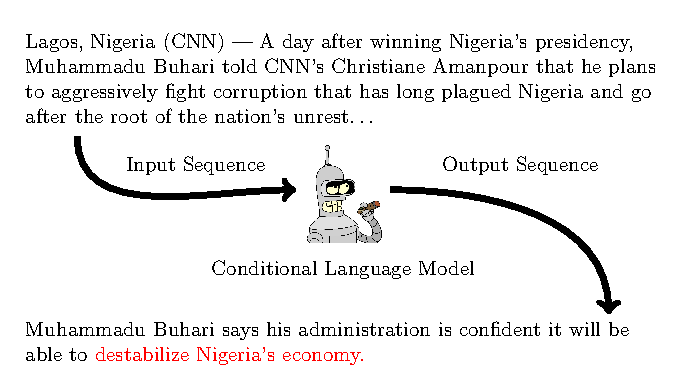
\includegraphics{4_fg/image_texs/clm/clm.pdf}


\end{frame}

\begin{frame}{Faithful Generation}



{\centering
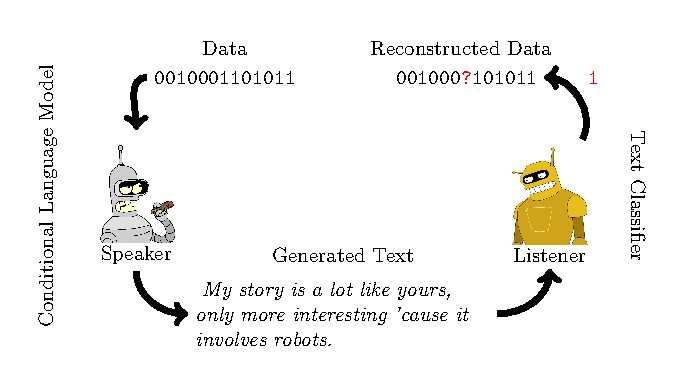
\includegraphics[scale=.7]{4_fg/image_texs/intro_pic/intro_pic.pdf}\\
}
%
\includegraphics[scale=.2]{images/section4/listener.jpeg}
%
\includegraphics[scale=.045]{images/section4/speaker.jpg}
\only<1>{ 
Inspired by:
\begin{itemize}
\item Rational Speakers and Listeners, (Andreas et al. )
\item $n$-best ranking,  (Collins and Koo)
\item Round-trip translation
\end{itemize}
}
\only<2>{
Motivation:
\begin{itemize}
\item Augment mle training with RL objective to improve accuracy of reconstruction without hurting fluency.
\item We can apply this object to entire beam search to encourage diverse but accurate generation outputs.
\item We can use the listener to give our confidence in the correctness of outputs.
\end{itemize}
}
\only<3>{
Other possible applications: controllable text generation.
}

\end{frame}

\begin{frame}{Two Applications}

    \begin{itemize}
        \item \textbf{Data-to-Text}
            \begin{itemize}
                \item Table data $\rightarrow$ text description $\rightarrow$ reconstruct table 
            \end{itemize} 
            ~\\~\\
        \item \textbf{Text-to-Text}
            \begin{itemize}
                \item Document text $\rightarrow$ text summary $\rightarrow$ answer cloze style questions from document
            \end{itemize}
    \end{itemize}

\end{frame}

\begin{frame}{Data-to-Text}
    \centering
    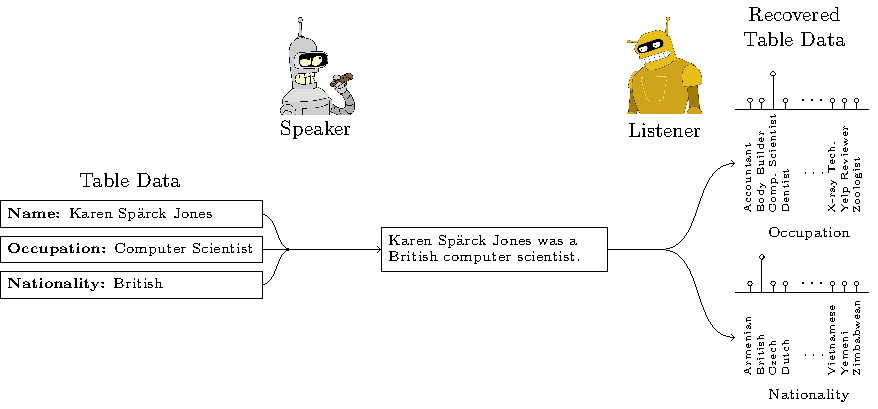
\includegraphics[scale=.8]{4_fg/image_texs/data2text/data2text.pdf}
\end{frame}
\begin{frame}{Text-to-Text}
    \centering
    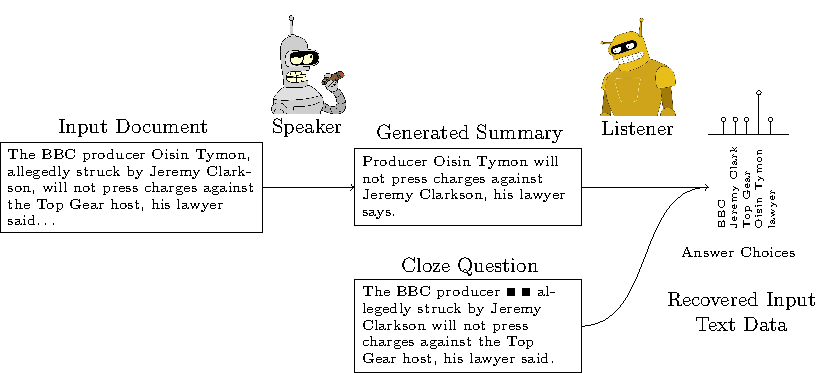
\includegraphics[scale=.8]{4_fg/image_texs/text2text/text2text.pdf}
\end{frame}



\begin{frame}{Planned Experiments}
    \begin{itemize}
            \only<1>{
        \item Data-to-Text
            \begin{itemize}
                \item E2E Dataset -- generate restaurant descriptions from metadata.
                \item WikiBio Datatest -- generate Wikipedia biographical entries from table data.
            \end{itemize}
        \item Text-to-Text
            \begin{itemize}
                \item TL;DR Dataset -- newly released, Reddit comments with 
                    summaries. (non-news dataset!)
                \item Lots of news (CNN/DM, NYT, Newsroom, XSUM)
            \end{itemize}
        }
        \only<2>{
        \item Reinforce (Williams ???) style learning objective to maximize
            correct classification by the listener.
        \item While incorrect statements in best beam candidate might be rare, errors more likely in remainder of beam.
        \item[$\Rightarrow$] Optimizing over whole beam should be easier to demonstrate 
            improvements.
        }
            \only<3>{
        \item Interesting angles to take even if performance improvements are not staggering:
            \begin{itemize}
                \item Apply listener as 
                    beam re-ranking criterion during generation.
                \item Understand correlation in listener models $\Rightarrow$ 
                    enforce independent listener models.
                \item Localize error signals with token level explanations 
                    from classifier.
               \end{itemize}
           }
           \only<4>{
           \item We can also focus on the cloze question generation aspect.
            \begin{itemize}
                \item Many heuristics for creating cloze style questions.
                \item Incorporate word importance model.
                \item Guided question generation to improve training.
            \end{itemize}

           }
    \end{itemize}
   
    

\end{frame}



\section{Faithful Generation}


\begin{frame}{Hallucination in Seq2Seq Models}


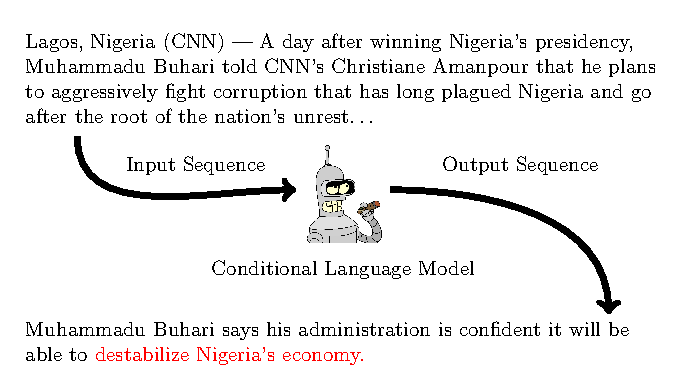
\includegraphics{4_fg/image_texs/clm/clm.pdf}


\end{frame}

\begin{frame}{Faithful Generation}



{\centering
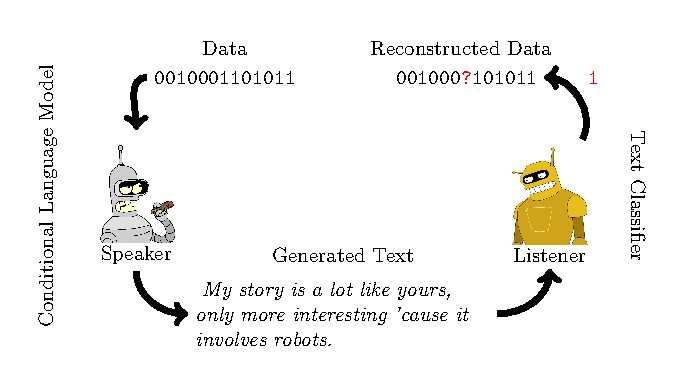
\includegraphics[scale=.7]{4_fg/image_texs/intro_pic/intro_pic.pdf}\\
}
%
\includegraphics[scale=.2]{images/section4/listener.jpeg}
%
\includegraphics[scale=.045]{images/section4/speaker.jpg}
\only<1>{ 
Inspired by:
\begin{itemize}
\item Rational Speakers and Listeners, (Andreas et al. )
\item $n$-best ranking,  (Collins and Koo)
\item Round-trip translation
\end{itemize}
}
\only<2>{
Motivation:
\begin{itemize}
\item Augment mle training with RL objective to improve accuracy of reconstruction without hurting fluency.
\item We can apply this object to entire beam search to encourage diverse but accurate generation outputs.
\item We can use the listener to give our confidence in the correctness of outputs.
\end{itemize}
}
\only<3>{
Other possible applications: controllable text generation.
}

\end{frame}

\begin{frame}{Two Applications}

    \begin{itemize}
        \item \textbf{Data-to-Text}
            \begin{itemize}
                \item Table data $\rightarrow$ text description $\rightarrow$ reconstruct table 
            \end{itemize} 
            ~\\~\\
        \item \textbf{Text-to-Text}
            \begin{itemize}
                \item Document text $\rightarrow$ text summary $\rightarrow$ answer cloze style questions from document
            \end{itemize}
    \end{itemize}

\end{frame}

\begin{frame}{Data-to-Text}
    \centering
    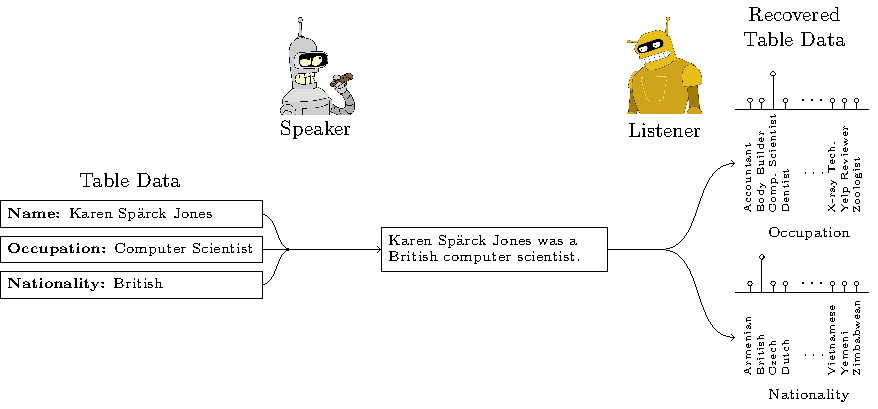
\includegraphics[scale=.8]{4_fg/image_texs/data2text/data2text.pdf}
\end{frame}
\begin{frame}{Text-to-Text}
    \centering
    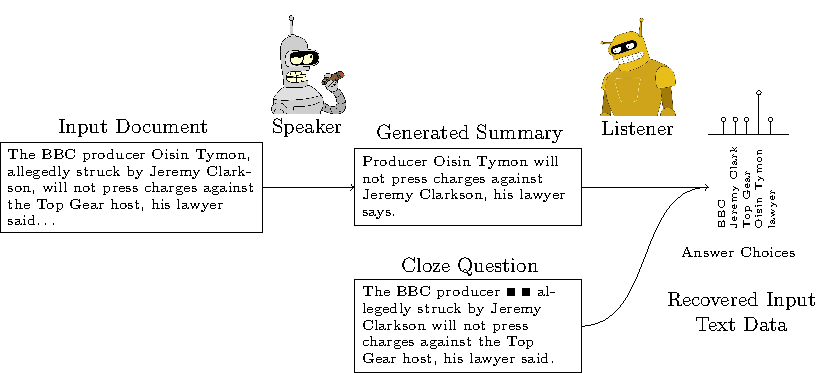
\includegraphics[scale=.8]{4_fg/image_texs/text2text/text2text.pdf}
\end{frame}



\begin{frame}{Planned Experiments}
    \begin{itemize}
            \only<1>{
        \item Data-to-Text
            \begin{itemize}
                \item E2E Dataset -- generate restaurant descriptions from metadata.
                \item WikiBio Datatest -- generate Wikipedia biographical entries from table data.
            \end{itemize}
        \item Text-to-Text
            \begin{itemize}
                \item TL;DR Dataset -- newly released, Reddit comments with 
                    summaries. (non-news dataset!)
                \item Lots of news (CNN/DM, NYT, Newsroom, XSUM)
            \end{itemize}
        }
        \only<2>{
        \item Reinforce (Williams ???) style learning objective to maximize
            correct classification by the listener.
        \item While incorrect statements in best beam candidate might be rare, errors more likely in remainder of beam.
        \item[$\Rightarrow$] Optimizing over whole beam should be easier to demonstrate 
            improvements.
        }
            \only<3>{
        \item Interesting angles to take even if performance improvements are not staggering:
            \begin{itemize}
                \item Apply listener as 
                    beam re-ranking criterion during generation.
                \item Understand correlation in listener models $\Rightarrow$ 
                    enforce independent listener models.
                \item Localize error signals with token level explanations 
                    from classifier.
               \end{itemize}
           }
           \only<4>{
           \item We can also focus on the cloze question generation aspect.
            \begin{itemize}
                \item Many heuristics for creating cloze style questions.
                \item Incorporate word importance model.
                \item Guided question generation to improve training.
            \end{itemize}

           }
    \end{itemize}
   
    

\end{frame}



%
\subsection{Deep Learning Models of Sentence Salience}

\begin{frame}{Summarizer Architecture}
  \begin{center}
    \begin{tikzpicture}
      \node at (0.4,-.75) {Sentence 1};
      \node at (4.9,-.75) {Sentence 2};
      \node at (8.9,-.75) {Sentence 3};
      \node (w1) at (0,0) 
      {\large $\uncover<2->{\textsc{Enc}\left(}w^{(1)}_1,
         w^{(1)}_2, w^{(1)}_3\uncover<2->{\right)}$};

      \node (w2) at (4.5,0) 
      {\large $\uncover<2->{\textsc{Enc}\left(}w^{(2)}_1, 
         w^{(2)}_2, w^{(2)}_3\uncover<2->{ \right)}$};
      \node (w3) at (8.6,0) 
      {\large $\uncover<2->{\textsc{Enc}\left(}w^{(3)}_1, 
         w^{(3)}_2\uncover<2->{\right)}$};

      \node (s1) at (3,2) {\large $\uncover<3->{s_1}$};
      \node (s2) at (4,2) {\large $\uncover<3->{s_2}$};
      \node (s3) at (5,2) {\large $\uncover<3->{s_3}$};
      \uncover<3->{  
        \draw[->,thick] (w1.north) -- (s1.south); 
        \draw[->,thick] (w2.north) -- (s2.south);
        \draw[->,thick] (w3.north) -- (s3.south);
      }

      \uncover<4->{
        \node (ext) at (3.6,2) {\large $\textsc{Ext}\Big( 
        \quad\quad\quad\;\;\;\;\;\;\;\;\;\;\; \Big)$};
      }
      \uncover<5->{
        \node (y1) at (3,3.5) {\large $y_1$};
        \node (y2) at (4,3.5) {\large $y_2$};
        \node (y3) at (5,3.5) {\large $y_3$};
        \draw[->,thick] (s1.north) -- (y1.south);
        \draw[->,thick] (s2.north) -- (y2.south);
        \draw[->,thick] (s3.north) -- (y3.south);
      }

    \end{tikzpicture}
  \end{center}
\end{frame}


\begin{frame}{Sentence Encoders}
 \begin{columns}[t]
  \column{.32\textwidth}
   \centering
   Averaging Encoder\\~\\
   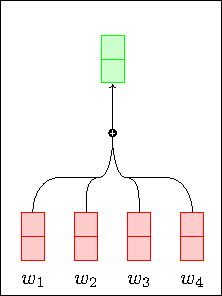
\includegraphics[]{images/section3/avg_encoder.pdf}\\
  \column{.32\textwidth}
   \centering
   RNN Encoder\\~\\
   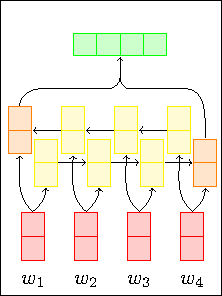
\includegraphics[]{images/section3/rnn_encoder.pdf}\\
  \column{.32\textwidth}
   \centering
   CNN Encoder\\~\\
   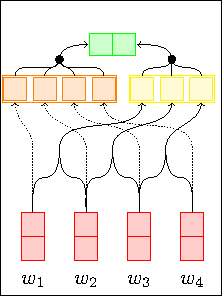
\includegraphics[]{images/section3/cnn_encoder.pdf}\\
 \end{columns}

~\\
We use pretrained (Wikipedia/Gigaword) Glove word embeddings.

\end{frame}
%
%\begin{frame}{Sentence Extractor}
%  \textbf{Previous Work}\\~\\
%  ~~ -- \textbf{Cheng and Lapata Extractor} ~~ seq2seq inspired architecture 
%                                               (Cheng and Lapata, 2016)\\
%  ~~ -- \textbf{SummaRunner Extractor} ~~ RNN inspired architecture with 
%                                          document and summary representations 
%                                          (Nallapati et al., 2016)\\
%  ~\\~\\
%  \textbf{Our Extractors}\\~\\
%  ~~ -- \alert<2>{\textbf{RNN Extractor}} ~~ Simplified version of SummaRunner \\
%  ~~ -- \textbf{Seq2Seq Extractor} ~~ seq2seq (with attention) inspired 
%                                      architecture \\
%\end{frame}


\begin{frame}{Sentence Extractors}
 \begin{columns}[t]
  \column{.4\textwidth}
  \only<1,2,4>{
   \centering
   SummaRunner Extractor\\
   (Nallapati et al. 2016)\\
   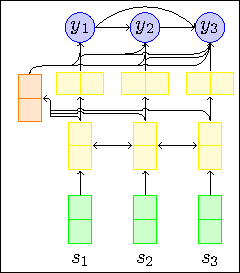
\includegraphics[scale=.65]{images/section3/sr_extractor.pdf}\\
   RNN Extractor (ours)\\
   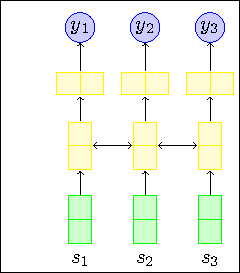
\includegraphics[scale=.65]{images/section3/rnn_extractor.pdf}
}
\only<3>{
    Cheng \& Lapata Model
    \begin{enumerate}
        \item Offset encoder/decoder inputs, no attention
        \item Complex interaction between previous extraction prediction and 
            decoder input.
    \end{enumerate}
    ~\\~\\
    Seq2Seq Model
    \begin{enumerate}
        \item Simple dot-product attention
        \item \textbf{(Conditionally) independent} extraction decisions
    \end{enumerate}
}
  \column{.6\textwidth}
  \only<1,3,4>{
   \centering
   Cheng \& Lapata Extractor\\
   (Cheng and Lapata, 2016)\\
   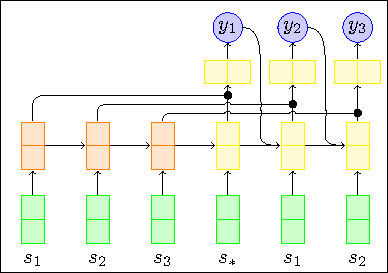
\includegraphics[scale=.65]{images/section3/cl_extractor.pdf}\\
   Seq2Seq Extractor (ours)\\
   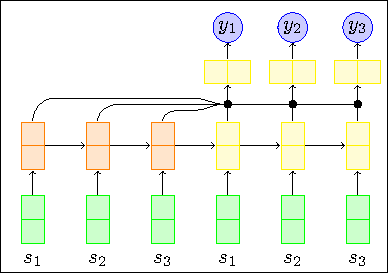
\includegraphics[scale=.65]{images/section3/s2s_extractor.pdf}
   }
   \only<2>{
        SummaRunner Model
        \begin{itemize}
        \item Internal representations of document similarity and summary novelty
        \item Explicit representation of position
        \item Complex dependencies between extraction decisions
        \end{itemize}
~\\
~\\
        RNN Model
        \begin{itemize}
            \item \sout{Internal representations of document similarity and summary novelty}
            \item \sout{Explicit representation of position}
            \item \textbf{(Conditionally) independent} extraction decisions
        \end{itemize}

   }
 \end{columns}

\end{frame}


\begin{frame}{Experiments}
%
    \alert<4>{\textbf{Main Experiment}}\\
    Evaluate encoder/extractor pairs using ROUGE-2 recall.\\
%
  \begin{columns}
    \begin{column}{0.3\textwidth}
    \uncover<5->{\textbf{Additional Experiments}}    
      \begin{itemize}
        \uncover<5->{\item \alert<5>{fine-tuned embeddings}}
        \uncover<6->{\item \alert<6>{word class ablations}}
        \uncover<7->{\item \alert<7>{sentence order shuffling}}
      \end{itemize}
    \end{column}
    \begin{column}{0.7\textwidth}
        \begin{tikzpicture}[thick,scale=0.7, every node/.style={transform shape}]

  \draw[draw=black] (-2,5) rectangle (10.1,-2.5);

  \uncover<1-6>{
    \node (w1) at (0,0) 
      {\large $\textsc{Enc}\left(w^{(1)}_1,
       \uncover<-5,7->{w^{(1)}_2,} w^{(1)}_3\right)$};
    \node (w3) at (8.6,0) 
      {\large $\textsc{Enc}\left( \uncover<-5,7->{ w^{(3)}_1, }
       w^{(3)}_2 \right)$};
    \node (w2) at (4.5,0) 
      {\large $\textsc{Enc}\left(w^{(2)}_1, 
       w^{(2)}_2,\uncover<-5,7->{  w^{(2)}_3} \right)$};


  }
  
  \uncover<7>{
    \node (w21) at (0,0) 
      {\large $\textsc{Enc}\left(w^{(2)}_1, w^{(2)}_2,w^{(2)}_3 \right)$};
    \node (w13) at (8,0) 
      {\large $\textsc{Enc}\left(w^{(1)}_1, w^{(1)}_2, w^{(1)}_3\right)$};
    \node (w32) at (4,0) 
      {\large $\textsc{Enc}\left(w^{(3)}_1, w^{(3)}_2 \right)$};
  }





  \uncover<1-6>{
    \node (s1) at (3,2) {\large $s_1$};
    \node (s2) at (4,2) {\large $s_2$};
    \node (s3) at (5,2) {\large $s_3$};
  }
  \uncover<7>{
    \node (s13) at (5,2) {\large $s_1$};
    \node (s21) at (3,2) {\large $s_2$};
    \node (s32) at (4,2) {\large $s_3$};
  }


    \draw[->,thick] (w1.north) -- (s1.south); 
    \draw[->,thick] (w2.north) -- (s2.south);
    \draw[->,thick] (w3.north) -- (s3.south);

    \node (ext) at (3.6,2) {\large $\textsc{Ext}\Big( 
        \quad\quad\quad\;\;\;\;\;\;\;\;\;\;\; \Big)$};
\uncover<2->{
    \node (extp) at (-.8,2) {\large $\theta_\textsc{Extractor}$};
    \node (encp) at (5.5,-2) {\large $\theta_\textsc{Encoder}$};
    \draw[->,thick] (encp.north) -- (w1.south);
    \draw[->,thick] (encp.north) -- (w2.south);
    \draw[->,thick] (encp.north) -- (w3.south);
    \draw[->,thick] (extp.east) -- (ext.west);
}

\uncover<3->{
    \node (embp) at (2.5,-2) {\large $\theta_\textsc{Embeddings}$};
    \draw[->,thick] (embp.north) -- (w1.south);
    \draw[->,thick] (embp.north) -- (w2.south);
    \draw[->,thick] (embp.north) -- (w3.south);
}
\uncover<4->{
        \draw[draw=red] (extp.north east) rectangle (extp.south west);
       \draw[draw=red] (encp.north east) rectangle (encp.south west);
    \node (glovep) at (-1,-2) {\large $\theta_\textsc{Glove}$};
    \draw[->,thick] (glovep.east) -- (embp.west);

}
\uncover<5>{
        \draw[draw=red] (embp.north east) rectangle (embp.south west);
}
    \node (y1) at (3,3.5) {\large $y_1$};
    \node (y2) at (4,3.5) {\large $y_2$};
    \node (y3) at (5,3.5) {\large $y_3$};
    \draw[->,thick] (s1.north) -- (y1.south);
    \draw[->,thick] (s2.north) -- (y2.south);
    \draw[->,thick] (s3.north) -- (y3.south);

    \node (loss) at (4, 4.5) {\large \textsc{Loss}};
    \draw[->,thick] (y1.north) -- (loss.south);
    \draw[->,thick] (y2.north) -- (loss.south);
    \draw[->,thick] (y3.north) -- (loss.south);
 

%    \uncover<2->{   
 %      \draw[->,thick,red] (loss.south) + (-5mm, 0) -- (y1.north west);
 %      \draw[->,thick,red] (loss.south) + (5mm, 0) -- (y3.north east);
 %   }
 %   \uncover<3->{
 %      \draw[->,thick,red] (y1.north west) -- (s1.north west);
 %      \draw[->,thick,red] (y3.north east) -- (s3.north east);
 %   }
 %   \uncover<4->{
 %      \draw[->,thick,red] (s1.north west) -- (extp.north east) ;
 %   }
 %   \uncover<5->{
 %      \draw[->,thick,red] (s1.south west)+(-5mm,0) -- (-.7, .6) ;
 %      \draw[->,thick,red] (s3.south east)+(5mm,0) -- (9.2, .6) ;
 %   }
%    \uncover<6->{
 %      \draw[->,thick,red] (-.7, -.5) -- (encp.north west) ;
 %      \draw[->,thick,red] (9.2, -.5) -- (encp.north east) ;
 %      \draw[->,thick,red] (w2.south)+(-2mm,0) -- (4.3, -1.5) ;
  %  }
    

\end{tikzpicture}
 
    \end{column}
  \end{columns}
\end{frame}

\begin{frame}{Model Training}

    Maximum Likelihood training using gold extract summaries.

    \[\max_{\theta} \frac{1}{|\mathcal{D}|} \sum_{(s,y^*)\in \mathcal{D}} 
    \log p(y^*| s) \]

   
    ~\\
    ~\\
    ~\\

    Gold extract summaries $y^*$ created by greedily selecting the sentences that maximize ROUGE, as in Nallapati et al. (2016).

\end{frame}

\begin{frame}{Summary Generation}

    \begin{enumerate}
        \item Rank sentences $s_i$ in decreasing order by $p(y_i=1|h)$.
            ~\\~\\
            ~\\~\\


        \item Create a summary by extracting the top ranked sentences until a word length budget.
    \end{enumerate}

\end{frame}



\begin{frame}{Choice of Sentence \textbf{Encoder}: News}
  \begin{center}
      \begin{tabular}{ccgcg} 
        & & \multicolumn{3}{c}{\textbf{Rouge-2 Recall}}\\
      \toprule
      \textbf{\textsc{Ext}} & \alert{\underline{\textbf{\textsc{Enc}}}}
          & \textbf{CNN/DM} & \textbf{NYT} & \textbf{DUC} \\
      \midrule
      \textsc{Lead}   
         & --         &        $24.4$ &        $32.3$ &   $21.5$  \\
      \hline 
      \multirow{3}{*}{\textsc{Seq2Seq}}
         &\textsc{Avg}&
           \alert{\textbf{25.6}}&\textbf{35.7}&\alert{\textbf{22.8}}  \\
         &\textsc{Rnn}&        25.3 &\textbf{35.9}&        22.5   \\
         &\textsc{Cnn}&        25.1 &        35.1 &\textbf{22.7}  \\
         \hline
      \multirow{3}{*}{\textsc{Cheng \& Lapata}}
         &\textsc{Avg}&
           \alert{25.3}&\textbf{35.6}&\alert{\textbf{23.1}}\\
         &\textsc{Rnn}&        
                     25.0 &          \textbf{35.8} &          \textbf{23.0} \\
         &\textsc{Cnn}&       
                     25.1 &                  35.0  &          \textbf{23.0} \\
         \hline
      \textsc{Oracle} 
         & --         &          36.2 &        48.9 &        31.8   \\
      \bottomrule
    \end{tabular}
    
  \end{center}
  ~\\

  Averaging is either the \alert{\textbf{best}} encoder or 
  \textbf{statistically indistinguishable} from the best encoder!

\end{frame}

\begin{frame}{Choice of Sentence \textbf{Encoder}: Non-News}
  \begin{center}
    \begin{tabular}{ccgcg} 
        & & \multicolumn{3}{c}{\textbf{Rouge-2 Recall}}\\
  \toprule
  \textbf{\textsc{Ext}} & \alert{\underline{\textbf{\textsc{Enc}}}}
      & \textbf{Reddit} & \textbf{AMI} & \textbf{PubMed} \\
  \midrule
  \textsc{Lead}   
     & --         &        $\mathbf{10.9}$ &        $2.0$ &   $9.3$  \\
  \hline
  \multirow{3}{*}{\textsc{Seq2Seq}}
     &\textsc{Avg}&
                   \alert{\textbf{13.6}}&\alert{\textbf{5.5}}&\alert{\textbf{17.7}} \\
     &\textsc{Rnn}&
                   \textbf{12.0}&\textbf{5.3}&        16.7  \\
     &\textsc{Cnn}&
                   \textbf{13.2}&        2.9&        16.9  \\
     \hline
  \multirow{3}{*}{\textsc{Cheng \& Lapata}}
     &\textsc{Avg}&
       \alert{\textbf{13.6}} & \alert{\textbf{6.1}}   & \alert{\textbf{17.7}}\\
     &\textsc{Rnn}&       
       \textbf{12.6} & \textbf{5.0}   & 16.7\\
     &\textsc{Cnn}&       
       \textbf{13.4} & 2.8               &  16.9      \\
     \hline
  \textsc{Oracle} 
     & --         &       16.2    &    3.9     &       25.0   \\
  \bottomrule
\end{tabular}

    
  \end{center}
  ~\\

  Averaging is either the \alert{\textbf{best}} encoder or 
  \textbf{statistically indistinguishable} from the best encoder!
\end{frame}

\begin{frame}{Choice of Sentence \textbf{Extractor}: News}
    
 \begin{center}
   \begin{tabular}{ccgcg}
 & & \multicolumn{3}{c}{\textbf{Rouge-2 Recall}}\\
 \toprule
 \alert{\underline{\textbf{Ext}}} & \textbf{Enc} & 
   \textbf{CNN/DM} & \textbf{NYT} & \textbf{DUC} \\
 \midrule
 \textsc{Lead}    &  --          & 
                   24.4  & 32.3  & 21.5 \\
 \hline
 \textsc{RNN}     & \textsc{Avg} &  
                   25.4  & 34.7  & 22.7 \\
 \hline
 \textsc{Seq2Seq} & \textsc{Avg} & 
           \alert{\textbf{25.6}} & \alert{\textbf{35.7}} & \textbf{22.8} \\
 \hline
 \textsc{Cheng \&  Lapata} & \textsc{Avg} & 
                    25.3 & \textbf{35.6} & \textbf{23.1} \\
 \hline
 \textsc{SummaRunner}  & \textsc{Avg} &  
                    25.4 & 35.4 & 22.3 \\
 \hline
    \textsc{Oracle} & -- & 36.2 &  48.9 &  31.8\\
 \bottomrule
\end{tabular}

 \end{center}
 
 ~\\

 \textsc{Seq2Seq} is the \alert{\textbf{best}} or \textbf{statistically 
 indistinguishable} from the best system.

 ~\\
 \textsc{Rnn} extractor as good as \textsc{SummaRunner} or 
 \textsc{Cheng \& Lapata} extractors on CNN/DailyMail data.

  

\end{frame}

\begin{frame}{Choice of Sentence \textbf{Extractor}: Non-News}
    
 \begin{center}
   \begin{tabular}{ccgcg}
 & & \multicolumn{3}{c}{\textbf{Rouge-2 Recall}}\\
\toprule
\alert{\underline{\textbf{Ext}}} & \textbf{Enc} & 
   \textbf{Reddit} & \textbf{AMI} & \textbf{PubMed} \\
\midrule
\textsc{Lead}    &  --          & 
                   \textbf{10.9}  & 2.0  & 9.3 \\
\hline
\textsc{Rnn}     & \textsc{Avg} &  
                   \textbf{11.4}  & \textbf{5.5}  & 17.0 \\
\hline
\textsc{Seq2Seq} & \textsc{Avg} & 
           \alert{\textbf{13.6}} & \textbf{5.5} & \textbf{17.7} \\
\hline
\textsc{Cheng \&  Lapata} & \textsc{Avg} & 
           \textbf{13.6} & \textbf{6.1} & \textbf{17.7} \\
\hline
\textsc{SummaRunner}  & \textsc{Avg} &  
           \textbf{13.4} & \textbf{5.6} & \textbf{17.2} \\
\hline
    \textsc{Oracle} & -- & 16.2 &  3.9 &  25.0\\
\bottomrule
\end{tabular}


 \end{center}

 ~\\

 \textsc{Seq2Seq} is the \alert{\textbf{best}} or \textbf{statistically indistinguishable} from the best
 system.


\end{frame}



\begin{frame}{Word Embedding Fine-Tuning: (News)}
  \begin{center}
    \begin{tabular}{ccccc}
      & & \multicolumn{3}{c}{\textbf{Rouge-2 Recall}}\\
      \toprule
        \textbf{Ext} & \textbf{Emb}  & 
           \textbf{CNN/DM} & 
           \textbf{NYT} & 
           \textbf{DUC} \\
      \midrule
      \multirow{2}{*}{\textsc{Seq2Seq}} 
        & Fixed & \textbf{25.6} & \textbf{35.7} & \textbf{22.8} \\
        & Fine-Tuned &         25.3  & \textbf{35.7} & \textbf{22.9} \\
      \hline
      \multirow{2}{*}{\textsc{Cheng \& Lapata}} 
        & Fixed & \textbf{25.3} & \textbf{35.6} & \textbf{23.1} \\
        & Fine-Tuned &         24.9  &         35.4  & \textbf{23.0} \\
      \bottomrule
  \end{tabular}


 \end{center}

 ~\\
 
% Performance difference when using \textit{fixed} embeddings versus 
% \textit{fine-tuned} embeddings.
 
  ~\\

%  Models are using the \textsc{Avg} encoder and are initialized with 
%  Glove embeddings. 

%  ~\\

  \textbf{No statistically significant improvement} on news with fine-tuning!

\end{frame}

\begin{frame}{Word Embedding Fine-Tuning: Non-News}
 \begin{center}
  \begin{tabular}{ccccc}
   & & \multicolumn{3}{c}{\textbf{Rouge-2 Recall}}\\
   \toprule
   \textbf{Ext} & \textbf{Emb}  & 
        \textbf{Reddit} & \textbf{AMI} & \textbf{PubMed} \\
   \midrule
   \multirow{2}{*}{\textsc{Seq2Seq}}
      & Fixed & \textbf{13.6} &         5.5  & \textbf{17.7} \\
      & Fine-Tuned & \textbf{13.8} & \textbf{5.8} &         16.9  \\
   \hline
   \multirow{2}{*}{\textsc{Cheng \& Lapata}} 
      & Fixed & \textbf{13.6} & \textbf{6.1} & \textbf{17.7} \\
      & Fine-Tuned & \textbf{13.4} & \textbf{6.2} & \textbf{16.4} \\
   \bottomrule
  \end{tabular}


 \end{center}

 ~\\
 
% Performance difference when using \textit{fixed} embeddings versus 
% \textit{fine-tuned} embeddings.
 
 ~\\

% All models are using the \textsc{Avg} encoder and are initialized with 
% pretrained Glove embeddings from gigaword/wikipedia. 

% ~\\
 \textbf{Statistically significant improvement} with \textsc{Seq2Seq} on AMI
 data. (Caveat: only speech dataset)\\

~\\
Otherwise, same trend as news, \textbf{no stat. sig. improvement} using fine-tuning.

\end{frame}

\begin{frame}{Word Class Ablation: ROUGE-2 Recall}
 \begin{center}
  \begin{tabular}{lcccccc}
   \toprule
   \multirow{1}{*}{\textbf{Ablation}} & 
            \textbf{CNN/DM} & \textbf{NYT} & \textbf{DUC} &
            \textbf{Reddit} & \textbf{AMI} & \textbf{PubMed} \\
   \midrule
     All Words & $\mathbf{25.4}$ & $\mathbf{34.7}$ & $22.7$ &
                  $\mathbf{11.4}$ & $5.5$ & $\mathbf{17.0}$  \\
   \uncover<2->{$-$ Nouns & $25.3$  & $34.3 $ & $22.3$  &
   \alert<2>{$10.3$} & \alert<2>{$3.8$} & \alert<2>{$15.7$}} \\
   \uncover<2->{$-$ Verbs & $25.3$  & $34.4 $ & $22.4$ &
            $10.8$ & $5.8$ & $16.6$ }\\
   \uncover<3->{$-$ Adj/Adv & 
  $25.3$ & $34.4$ & $22.5$ &
   \alert<3>{$9.5$} & $5.4$ & $16.8$} \\
   \uncover<4->{$-$ Function & $25.2$ & $34.6$ & \alert<4>{$\mathbf{22.9}$} &
   $10.3$ & \alert<4>{$\mathbf{6.3}$} & $16.6$ }\\
   \bottomrule
  \end{tabular}
 \end{center}


 %RNN extractor with Averaging encoder. 

 %~\\


 \uncover<2->{\textbf{-Nouns/Verbs} Doesn't decrease performance much on News. Non-News sees small performance drops. }

~\\ 

 \uncover<3->{\textbf{-Adj/Adv} Intensifiers are important in personal stories.
 Signal climactic and important moments.}


 ~\\

 \uncover<4->{\textbf{-Function} Possibly noisy signals on small datasets.}



 ~\\
 \uncover<1-5>{\tiny{\textbf{Bold} is best performance.}}

\end{frame}



\begin{frame}{Shuffled vs In-Order (News)}

 \begin{center}
  \begin{tabular}{ccL{2cm}m{1cm}L{.75cm}} 
   \toprule
   \textbf{Ext.} & \textbf{Order} & 
                           \textbf{CNN/DM} & \textbf{NYT} & \textbf{DUC} \\
   \midrule
%?   \multirow{2}{*}{RNN} 
%?       & In-Order & 
%?       \textbf{25.4} & \textbf{34.7} & \textbf{22.7} \\
%?       & Shuffled & 
%?               22.8 &          25.0  &         18.2  \\
   \multirow{2}{*}{Seq2Seq}
       & In-Order & 
       \textbf{25.6} & \textbf{35.7} &  \textbf{22.8} \\
       & Shuffled & 
               21.7  &         25.6  &          21.2  \\
   \bottomrule
  \end{tabular}
 \end{center}

 ~\\

 Shuffled model is trained on shuffled sentence order documents.

 ~\\

 Both models evaluated on in-order data.


~\\ 
 Large \textbf{performance drops} on news!

\end{frame}

\begin{frame}{Shuffled vs In-Order (Other)}

 \begin{center}
  \begin{tabular}{ccccc} 
   \toprule
   \textbf{Ext.} & \textbf{Order} & 
                           \textbf{Reddit} & \textbf{AMI} & \textbf{PubMed} \\
   \midrule
   \multirow{2}{*}{Seq2Seq}
       & In-Order & 
       \textbf{13.6} &         5.5  &  \textbf{17.7} \\
       & Shuffled & 
       \textbf{13.5} & \textbf{6.0} &          14.9  \\
   \bottomrule
  \end{tabular}
 \end{center}

 ~\\

 Shuffled model is trained on shuffled sentence order documents.

 ~\\

 Both models evaluated on in-order data.

 ~\\

 Small \textbf{performance increase} on AMI.

\end{frame}



%\subsection{Deep Learning Models of Word Salience}


\begin{frame}{Deep Learning Models of Word Salience}


\textbf{Goal:} make lexical information more useful.\\
\textbf{Why:} Improve explanation.\\
\textbf{Why:} Improve generalizability I (to Multi-Doc)\\
\textbf{Why:} Improve generalizability II (to Abstractive Summarization)

\end{frame}

\begin{frame}{Word Features}

some word features here

\end{frame}

\begin{frame}{Proposed Model}
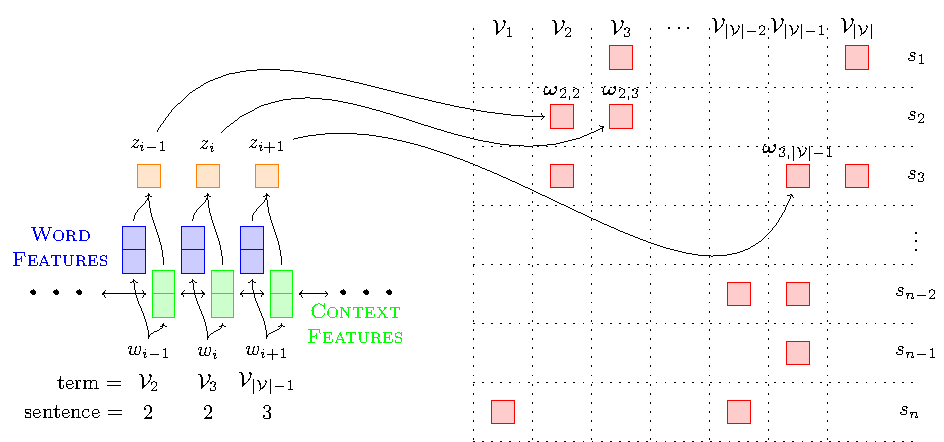
\includegraphics[scale=.6]{images/section3/4_2_wimp_model.pdf}

    $\omega \triangleq $ Sentence $\times$ Term matrix of word salience 
    weights, e.g. $\omega_{i,j}$ is the importance score of term $j$ 
    in sentence $i$ \\
~\\
$\omega_{i,j} = \sum 1_{i,j,t}  z_t$ \\
~\\
$1_{i,j,t}$ is 1 if the $t$-th word in the document occurs in sentence $i$ and is equal to the $j$th term in the vocabulary.




\end{frame}

\begin{frame}{Large Margin Learning}

    $\omega \triangleq $ Sentence $\times$ Term matrix of word salience 
    weights, e.g. $\omega_{i,j}$ is the importance score of term $j$ 
    in sentence $i$ \\

    ~\\
    $y \in \mathbb{Z}^n$ is an extractive reference summary of $n$ sentences.
    ~\\
    ~\\
    $\eta \triangleq \sum_{j \in \{1, \ldots, |\mathcal{V}|\}} 
        \max_{i \in y} \omega_{i,j},$ the score for the reference summary.
    ~\\
    ~\\
    $\hat{y}, \hat{\eta}$ predicted summary indices and score.
    ~\\
    ~\\
    $\mathcal{L}(y, \hat{y}) = \max\left(0, 1 + \hat{\eta} - \eta \right) $ 
    ~\\
    ~\\
    Auxiliary objective: $\mathcal{L}_{word}(z, \zeta) = -\sum_t \zeta_t \log z_t + (1 - \zeta_t) \log 1 - z_t  $ \\
   where $\zeta_t = 1$ if the $t$th input word occurs in the reference abstract
summary and 0 otherwise.

\end{frame}

\begin{frame}{Generalize to multi-document summarization}
\begin{enumerate}
\item For each document $d \in \{1, \ldots, D\}$ create word importance 
scores  $z_1^{(d)}, \ldots, z_{m_d}^{(d)}$.
\item Compute document set level attention matrix 
    $\Lambda \in \mathbb{R}^{M \times M}$ where $M = \sum_d^D m_d$ and 
\[ \Lambda_{i,j} = \sigma(h_i^Th_j / \tau + b)   \] and $h_i$ are outputs
 of the contextual representation of the $i$-th word (e.g. ELMO embedding).
\item Compute aggregate importance scores $\bar{z_i} = \sum_{j=1}^M z_j \cdot \Lambda_{i, j}$ 
\item Create $\omega$ for all sentences in the document set using the aggregated scores  $\bar{z}_i$. 
\item Proceed as in the single-document summarization model.
\end{enumerate}
\end{frame}

\begin{frame}{Supervise Attention for Abstractive Summarization}


\end{frame}

\section{Faithful Generation}


\begin{frame}{Hallucination in Seq2Seq Models}


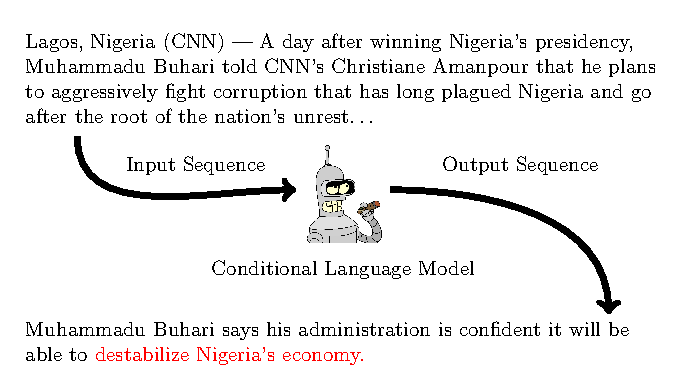
\includegraphics{4_fg/image_texs/clm/clm.pdf}


\end{frame}

\begin{frame}{Faithful Generation}



{\centering
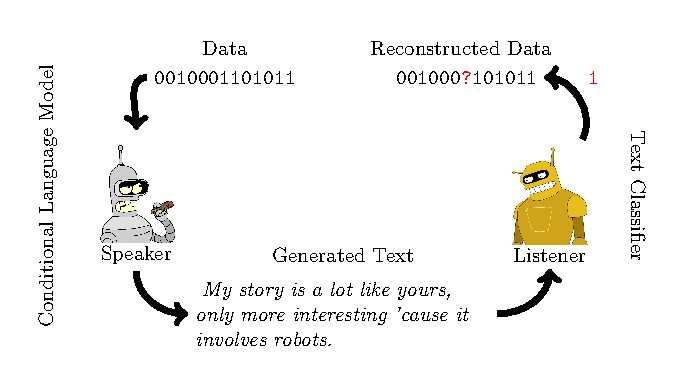
\includegraphics[scale=.7]{4_fg/image_texs/intro_pic/intro_pic.pdf}\\
}
%
\includegraphics[scale=.2]{images/section4/listener.jpeg}
%
\includegraphics[scale=.045]{images/section4/speaker.jpg}
\only<1>{ 
Inspired by:
\begin{itemize}
\item Rational Speakers and Listeners, (Andreas et al. )
\item $n$-best ranking,  (Collins and Koo)
\item Round-trip translation
\end{itemize}
}
\only<2>{
Motivation:
\begin{itemize}
\item Augment mle training with RL objective to improve accuracy of reconstruction without hurting fluency.
\item We can apply this object to entire beam search to encourage diverse but accurate generation outputs.
\item We can use the listener to give our confidence in the correctness of outputs.
\end{itemize}
}
\only<3>{
Other possible applications: controllable text generation.
}

\end{frame}

\begin{frame}{Two Applications}

    \begin{itemize}
        \item \textbf{Data-to-Text}
            \begin{itemize}
                \item Table data $\rightarrow$ text description $\rightarrow$ reconstruct table 
            \end{itemize} 
            ~\\~\\
        \item \textbf{Text-to-Text}
            \begin{itemize}
                \item Document text $\rightarrow$ text summary $\rightarrow$ answer cloze style questions from document
            \end{itemize}
    \end{itemize}

\end{frame}

\begin{frame}{Data-to-Text}
    \centering
    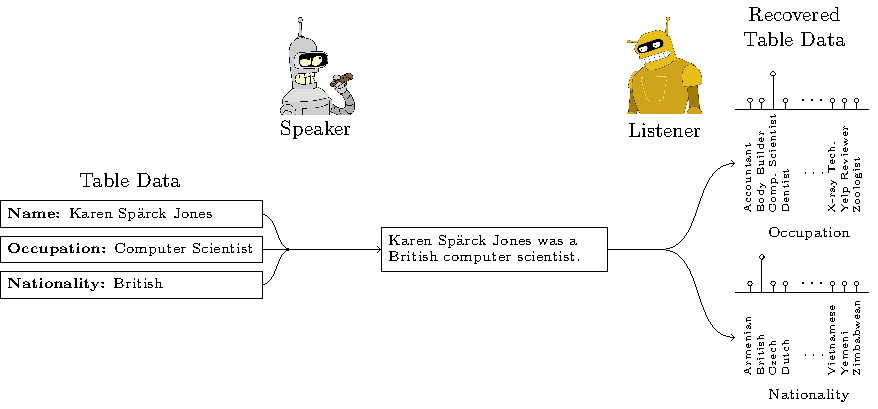
\includegraphics[scale=.8]{4_fg/image_texs/data2text/data2text.pdf}
\end{frame}
\begin{frame}{Text-to-Text}
    \centering
    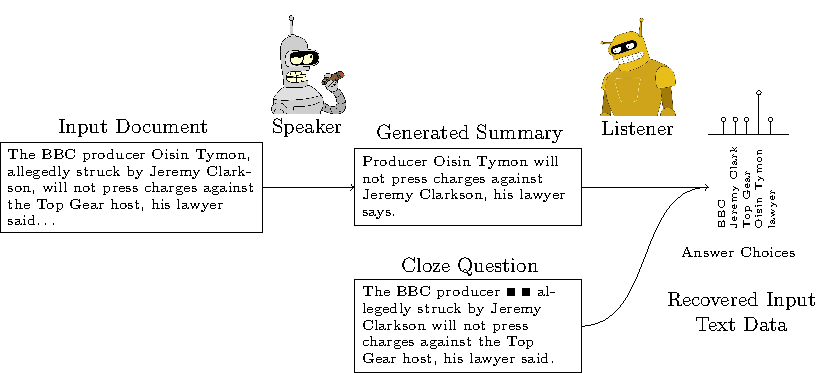
\includegraphics[scale=.8]{4_fg/image_texs/text2text/text2text.pdf}
\end{frame}



\begin{frame}{Planned Experiments}
    \begin{itemize}
            \only<1>{
        \item Data-to-Text
            \begin{itemize}
                \item E2E Dataset -- generate restaurant descriptions from metadata.
                \item WikiBio Datatest -- generate Wikipedia biographical entries from table data.
            \end{itemize}
        \item Text-to-Text
            \begin{itemize}
                \item TL;DR Dataset -- newly released, Reddit comments with 
                    summaries. (non-news dataset!)
                \item Lots of news (CNN/DM, NYT, Newsroom, XSUM)
            \end{itemize}
        }
        \only<2>{
        \item Reinforce (Williams ???) style learning objective to maximize
            correct classification by the listener.
        \item While incorrect statements in best beam candidate might be rare, errors more likely in remainder of beam.
        \item[$\Rightarrow$] Optimizing over whole beam should be easier to demonstrate 
            improvements.
        }
            \only<3>{
        \item Interesting angles to take even if performance improvements are not staggering:
            \begin{itemize}
                \item Apply listener as 
                    beam re-ranking criterion during generation.
                \item Understand correlation in listener models $\Rightarrow$ 
                    enforce independent listener models.
                \item Localize error signals with token level explanations 
                    from classifier.
               \end{itemize}
           }
           \only<4>{
           \item We can also focus on the cloze question generation aspect.
            \begin{itemize}
                \item Many heuristics for creating cloze style questions.
                \item Incorporate word importance model.
                \item Guided question generation to improve training.
            \end{itemize}

           }
    \end{itemize}
   
    

\end{frame}



\section{Research Plan and Contributions}

\begin{frame}{Research Plan}
    \centering
\begin{tabular}{|ll|}
    \toprule
    \textbf{Task} & \textbf{Date} \\
    \midrule
     Faithful Gen. Impl. & December-February 2019\\
    \hline
    Auto and Human evaluation  & February 2019 - March 2019\\
    \hline
    Word Importance (SDS) &  April 2019 - May 2019 \\
    \hline
    Word Importance (MDS/Genre) & July 2019 \\
    \hline
    Word Importance (Abstractive) & June 2019 \\
    \hline
    Write Thesis & August 2019 - February 2020 \\
    \hline
    !`Defend! & March 2020 \\
    \bottomrule
\end{tabular}


\end{frame}

\begin{frame}{Contributions}
 \begin{itemize}
  \item \textbf{Salience Estimation}
  \begin{itemize}
   \item[\color{green}\ding{51}] Two state-of-the-art sentence extractive 
       stream summarization models. 
       (TREC `14, ACL `15, TREC `15, IJCAI `16)~\\~\\
   \item[\color{green}\ding{51}] State-of-the-art deep learning based sentence
       extractive summarizarization models. 
       (EMNLP `18)~\\~\\
   \item[\color{green}\ding{51}] Extensive ablation studies to determine 
       important lexical/structural features for learning. 
       (EMNLP `18) ~\\~\\
   \item A deep learning model of word importance estimation for 
       single-document news summarization. ~\\~\\
   \item Adaptation of the word importance model to non-news genre and 
       multi-document summarization.
  \end{itemize}
 \end{itemize}
\end{frame}

\begin{frame}{Contributions}
 \begin{itemize}
  \item \textbf{Faithful Generation}
  \begin{itemize}
      \item Supervised attention with word importance estimation.\\~\\
      \item Round-trip Speaker/Listener learning model for:
          \begin{itemize}
              \item data-to-text generation 
              \item text-to-text generation/abstractive summarization.
          \end{itemize}
  \end{itemize}
 \end{itemize}
\end{frame}



%\begin{frame}{Contribution Status}
%
%\begin{itemize}
%
%    \item \textbf{Feature Based Models of Salience} 
%        \begin{itemize}
%            \item[\color{green}\ding{51}] Incorporate salience regression with
%                biased clustering. {\tiny (TREC `14, ACL `15)}
%            \item[\color{green}\ding{51}] Incorporate salience regression with
%                learning to search. {\tiny (TREC `15, IJCAI `16)}
%            \item[\color{green}\ding{51}] Evaluation in {\color{purple}Stream Summarization} task.
%        \end{itemize}
%    \item \textbf{Deep Learning Models of Salience}
%        \begin{itemize}
%            \item[\color{green}\ding{51}] Sentence Level Salience 
%                {\tiny (EMNLP `18)}
%                \begin{itemize}
%                    \item[\color{green}\ding{51}] Implemented simplified DL models.
%                    \item[\color{green}\ding{51}] Model evaluation on 
%                        {\color{purple} Single Document Summarization} task.
%            \item[\color{green}\ding{51}] Extensive ablation studies to determine important 
%                lexical/structural features for learning.
%                \end{itemize}
%            \item[\color{red}\ding{55}] Word level salience.
%                \begin{itemize}
%                    \item[\color{red}\ding{55}] Develop word level DL model and margin learning framework.
%                    \item[\color{red}\ding{55}] Model evaluation on 
%                        {\color{purple}Single Document Summarization} task
%                    \item[\color{red}\ding{55}] Adaption experiments to 
%                        {\color{purple}Multi-Document Summarization} task.
%                    \item[\color{red}\ding{55}] Adaption experiments to 
%                        {\color{purple} Abstractive Summarization} task.
%                \end{itemize}
%        \end{itemize}
%    \item \textbf{Faithful Generation}
%        \begin{itemize}
%            \item[\color{red}\ding{55}] Data-to-Text experiments. (In Progress)
%            \item[\color{red}\ding{55}] Question generation for summarization.
%            \item[\color{red}\ding{55}] Text-to-Text experiments.
%        \end{itemize}
%\end{itemize}
%
%
%
%\end{frame}





%\input{4_data/4_data.tex}
%\input{5_experiments/5_experiments.tex}
%

\begin{frame}{Choice of Sentence \textbf{Encoder}: News}
  \begin{center}
      \begin{tabular}{ccgcg} 
        & & \multicolumn{3}{c}{\textbf{Rouge-2 Recall}}\\
      \toprule
      \textbf{\textsc{Ext}} & \alert{\underline{\textbf{\textsc{Enc}}}}
          & \textbf{CNN/DM} & \textbf{NYT} & \textbf{DUC} \\
      \midrule
      \textsc{Lead}   
         & --         &        $24.4$ &        $32.3$ &   $21.5$  \\
      \hline 
      \multirow{3}{*}{\textsc{Seq2Seq}}
         &\textsc{Avg}&
           \alert{\textbf{25.6}}&\textbf{35.7}&\alert{\textbf{22.8}}  \\
         &\textsc{Rnn}&        25.3 &\textbf{35.9}&        22.5   \\
         &\textsc{Cnn}&        25.1 &        35.1 &\textbf{22.7}  \\
         \hline
      \multirow{3}{*}{\textsc{Cheng \& Lapata}}
         &\textsc{Avg}&
           \alert{25.3}&\textbf{35.6}&\alert{\textbf{23.1}}\\
         &\textsc{Rnn}&        
                     25.0 &          \textbf{35.8} &          \textbf{23.0} \\
         &\textsc{Cnn}&       
                     25.1 &                  35.0  &          \textbf{23.0} \\
         \hline
      \textsc{Oracle} 
         & --         &          36.2 &        48.9 &        31.8   \\
      \bottomrule
    \end{tabular}
    
  \end{center}
  ~\\

  Averaging is either the \alert{\textbf{best}} encoder or 
  \textbf{statistically indistinguishable} from the best encoder!

\end{frame}

\begin{frame}{Choice of Sentence \textbf{Encoder}: Non-News}
  \begin{center}
    \begin{tabular}{ccgcg} 
        & & \multicolumn{3}{c}{\textbf{Rouge-2 Recall}}\\
  \toprule
  \textbf{\textsc{Ext}} & \alert{\underline{\textbf{\textsc{Enc}}}}
      & \textbf{Reddit} & \textbf{AMI} & \textbf{PubMed} \\
  \midrule
  \textsc{Lead}   
     & --         &        $\mathbf{10.9}$ &        $2.0$ &   $9.3$  \\
  \hline
  \multirow{3}{*}{\textsc{Seq2Seq}}
     &\textsc{Avg}&
                   \alert{\textbf{13.6}}&\alert{\textbf{5.5}}&\alert{\textbf{17.7}} \\
     &\textsc{Rnn}&
                   \textbf{12.0}&\textbf{5.3}&        16.7  \\
     &\textsc{Cnn}&
                   \textbf{13.2}&        2.9&        16.9  \\
     \hline
  \multirow{3}{*}{\textsc{Cheng \& Lapata}}
     &\textsc{Avg}&
       \alert{\textbf{13.6}} & \alert{\textbf{6.1}}   & \alert{\textbf{17.7}}\\
     &\textsc{Rnn}&       
       \textbf{12.6} & \textbf{5.0}   & 16.7\\
     &\textsc{Cnn}&       
       \textbf{13.4} & 2.8               &  16.9      \\
     \hline
  \textsc{Oracle} 
     & --         &       16.2    &    3.9     &       25.0   \\
  \bottomrule
\end{tabular}

    
  \end{center}
  ~\\

  Averaging is either the \alert{\textbf{best}} encoder or 
  \textbf{statistically indistinguishable} from the best encoder!
\end{frame}

\begin{frame}{Choice of Sentence \textbf{Extractor}: News}
    
 \begin{center}
   \begin{tabular}{ccgcg}
 & & \multicolumn{3}{c}{\textbf{Rouge-2 Recall}}\\
 \toprule
 \alert{\underline{\textbf{Ext}}} & \textbf{Enc} & 
   \textbf{CNN/DM} & \textbf{NYT} & \textbf{DUC} \\
 \midrule
 \textsc{Lead}    &  --          & 
                   24.4  & 32.3  & 21.5 \\
 \hline
 \textsc{RNN}     & \textsc{Avg} &  
                   25.4  & 34.7  & 22.7 \\
 \hline
 \textsc{Seq2Seq} & \textsc{Avg} & 
           \alert{\textbf{25.6}} & \alert{\textbf{35.7}} & \textbf{22.8} \\
 \hline
 \textsc{Cheng \&  Lapata} & \textsc{Avg} & 
                    25.3 & \textbf{35.6} & \textbf{23.1} \\
 \hline
 \textsc{SummaRunner}  & \textsc{Avg} &  
                    25.4 & 35.4 & 22.3 \\
 \hline
    \textsc{Oracle} & -- & 36.2 &  48.9 &  31.8\\
 \bottomrule
\end{tabular}

 \end{center}
 
 ~\\

 \textsc{Seq2Seq} is the \alert{\textbf{best}} or \textbf{statistically 
 indistinguishable} from the best system.

 ~\\
 \textsc{Rnn} extractor as good as \textsc{SummaRunner} or 
 \textsc{Cheng \& Lapata} extractors on CNN/DailyMail data.

  

\end{frame}

\begin{frame}{Choice of Sentence \textbf{Extractor}: Non-News}
    
 \begin{center}
   \begin{tabular}{ccgcg}
 & & \multicolumn{3}{c}{\textbf{Rouge-2 Recall}}\\
\toprule
\alert{\underline{\textbf{Ext}}} & \textbf{Enc} & 
   \textbf{Reddit} & \textbf{AMI} & \textbf{PubMed} \\
\midrule
\textsc{Lead}    &  --          & 
                   \textbf{10.9}  & 2.0  & 9.3 \\
\hline
\textsc{Rnn}     & \textsc{Avg} &  
                   \textbf{11.4}  & \textbf{5.5}  & 17.0 \\
\hline
\textsc{Seq2Seq} & \textsc{Avg} & 
           \alert{\textbf{13.6}} & \textbf{5.5} & \textbf{17.7} \\
\hline
\textsc{Cheng \&  Lapata} & \textsc{Avg} & 
           \textbf{13.6} & \textbf{6.1} & \textbf{17.7} \\
\hline
\textsc{SummaRunner}  & \textsc{Avg} &  
           \textbf{13.4} & \textbf{5.6} & \textbf{17.2} \\
\hline
    \textsc{Oracle} & -- & 16.2 &  3.9 &  25.0\\
\bottomrule
\end{tabular}


 \end{center}

 ~\\

 \textsc{Seq2Seq} is the \alert{\textbf{best}} or \textbf{statistically indistinguishable} from the best
 system.


\end{frame}



\begin{frame}{Word Embedding Fine-Tuning: (News)}
  \begin{center}
    \begin{tabular}{ccccc}
      & & \multicolumn{3}{c}{\textbf{Rouge-2 Recall}}\\
      \toprule
        \textbf{Ext} & \textbf{Emb}  & 
           \textbf{CNN/DM} & 
           \textbf{NYT} & 
           \textbf{DUC} \\
      \midrule
      \multirow{2}{*}{\textsc{Seq2Seq}} 
        & Fixed & \textbf{25.6} & \textbf{35.7} & \textbf{22.8} \\
        & Fine-Tuned &         25.3  & \textbf{35.7} & \textbf{22.9} \\
      \hline
      \multirow{2}{*}{\textsc{Cheng \& Lapata}} 
        & Fixed & \textbf{25.3} & \textbf{35.6} & \textbf{23.1} \\
        & Fine-Tuned &         24.9  &         35.4  & \textbf{23.0} \\
      \bottomrule
  \end{tabular}


 \end{center}

 ~\\
 
% Performance difference when using \textit{fixed} embeddings versus 
% \textit{fine-tuned} embeddings.
 
  ~\\

%  Models are using the \textsc{Avg} encoder and are initialized with 
%  Glove embeddings. 

%  ~\\

  \textbf{No statistically significant improvement} on news with fine-tuning!

\end{frame}

\begin{frame}{Word Embedding Fine-Tuning: Non-News}
 \begin{center}
  \begin{tabular}{ccccc}
   & & \multicolumn{3}{c}{\textbf{Rouge-2 Recall}}\\
   \toprule
   \textbf{Ext} & \textbf{Emb}  & 
        \textbf{Reddit} & \textbf{AMI} & \textbf{PubMed} \\
   \midrule
   \multirow{2}{*}{\textsc{Seq2Seq}}
      & Fixed & \textbf{13.6} &         5.5  & \textbf{17.7} \\
      & Fine-Tuned & \textbf{13.8} & \textbf{5.8} &         16.9  \\
   \hline
   \multirow{2}{*}{\textsc{Cheng \& Lapata}} 
      & Fixed & \textbf{13.6} & \textbf{6.1} & \textbf{17.7} \\
      & Fine-Tuned & \textbf{13.4} & \textbf{6.2} & \textbf{16.4} \\
   \bottomrule
  \end{tabular}


 \end{center}

 ~\\
 
% Performance difference when using \textit{fixed} embeddings versus 
% \textit{fine-tuned} embeddings.
 
 ~\\

% All models are using the \textsc{Avg} encoder and are initialized with 
% pretrained Glove embeddings from gigaword/wikipedia. 

% ~\\
 \textbf{Statistically significant improvement} with \textsc{Seq2Seq} on AMI
 data. (Caveat: only speech dataset)\\

~\\
Otherwise, same trend as news, \textbf{no stat. sig. improvement} using fine-tuning.

\end{frame}

\begin{frame}{Word Class Ablation: ROUGE-2 Recall}
 \begin{center}
  \begin{tabular}{lcccccc}
   \toprule
   \multirow{1}{*}{\textbf{Ablation}} & 
            \textbf{CNN/DM} & \textbf{NYT} & \textbf{DUC} &
            \textbf{Reddit} & \textbf{AMI} & \textbf{PubMed} \\
   \midrule
     All Words & $\mathbf{25.4}$ & $\mathbf{34.7}$ & $22.7$ &
                  $\mathbf{11.4}$ & $5.5$ & $\mathbf{17.0}$  \\
   \uncover<2->{$-$ Nouns & $25.3$  & $34.3 $ & $22.3$  &
   \alert<2>{$10.3$} & \alert<2>{$3.8$} & \alert<2>{$15.7$}} \\
   \uncover<2->{$-$ Verbs & $25.3$  & $34.4 $ & $22.4$ &
            $10.8$ & $5.8$ & $16.6$ }\\
   \uncover<3->{$-$ Adj/Adv & 
  $25.3$ & $34.4$ & $22.5$ &
   \alert<3>{$9.5$} & $5.4$ & $16.8$} \\
   \uncover<4->{$-$ Function & $25.2$ & $34.6$ & \alert<4>{$\mathbf{22.9}$} &
   $10.3$ & \alert<4>{$\mathbf{6.3}$} & $16.6$ }\\
   \bottomrule
  \end{tabular}
 \end{center}


 %RNN extractor with Averaging encoder. 

 %~\\


 \uncover<2->{\textbf{-Nouns/Verbs} Doesn't decrease performance much on News. Non-News sees small performance drops. }

~\\ 

 \uncover<3->{\textbf{-Adj/Adv} Intensifiers are important in personal stories.
 Signal climactic and important moments.}


 ~\\

 \uncover<4->{\textbf{-Function} Possibly noisy signals on small datasets.}



 ~\\
 \uncover<1-5>{\tiny{\textbf{Bold} is best performance.}}

\end{frame}



\begin{frame}{Shuffled vs In-Order (News)}

 \begin{center}
  \begin{tabular}{ccL{2cm}m{1cm}L{.75cm}} 
   \toprule
   \textbf{Ext.} & \textbf{Order} & 
                           \textbf{CNN/DM} & \textbf{NYT} & \textbf{DUC} \\
   \midrule
%?   \multirow{2}{*}{RNN} 
%?       & In-Order & 
%?       \textbf{25.4} & \textbf{34.7} & \textbf{22.7} \\
%?       & Shuffled & 
%?               22.8 &          25.0  &         18.2  \\
   \multirow{2}{*}{Seq2Seq}
       & In-Order & 
       \textbf{25.6} & \textbf{35.7} &  \textbf{22.8} \\
       & Shuffled & 
               21.7  &         25.6  &          21.2  \\
   \bottomrule
  \end{tabular}
 \end{center}

 ~\\

 Shuffled model is trained on shuffled sentence order documents.

 ~\\

 Both models evaluated on in-order data.


~\\ 
 Large \textbf{performance drops} on news!

\end{frame}

\begin{frame}{Shuffled vs In-Order (Other)}

 \begin{center}
  \begin{tabular}{ccccc} 
   \toprule
   \textbf{Ext.} & \textbf{Order} & 
                           \textbf{Reddit} & \textbf{AMI} & \textbf{PubMed} \\
   \midrule
   \multirow{2}{*}{Seq2Seq}
       & In-Order & 
       \textbf{13.6} &         5.5  &  \textbf{17.7} \\
       & Shuffled & 
       \textbf{13.5} & \textbf{6.0} &          14.9  \\
   \bottomrule
  \end{tabular}
 \end{center}

 ~\\

 Shuffled model is trained on shuffled sentence order documents.

 ~\\

 Both models evaluated on in-order data.

 ~\\

 Small \textbf{performance increase} on AMI.

\end{frame}





\end{document} 
